\section{Rendu : Stratégie et conception}

\subsection{Stratégie de rendu d'un état}

Afin de pouvoir réaliser un rendu imagé de notre jeu RISK, il nous faut tout d’abord réaliser un rendu des différents éléments qui composent notre jeu. 

Comme pour la mise en place des différents états, nous allons différencier le rendu des éléments fixes (à savoir la map du jeu avec les pays et les continents) et le rendu des éléments mobiles amenés à se déplacer pendant le jeu (à savoir les armées et les cartes). 

Pour cela, le choix s'oriente vers une stratégie assez bas niveau et relativement proche du fonctionnement des unités graphiques. Plus précisément, le découpage se fait en différents plans nommés layers. Naturellement, un plan concernera les éléments statiques et affichera donc la carte, un autre sera consacré aux armées et un dernier s'occupera des cartes.

Pour la carte, le monde et la division des différents pays a été réalisé au préalable sur Tiled. Nous pouvons donc charger le fichier image comme texture et utiliser un sprite pour l'afficher dans la fenêtre du jeu. Nous pourrons ainsi redimensionner la carte principale comme nous le souhaitons.
Le second plan contiendra deux informations de bas niveau à savoir les textures contenant les tuiles et une unique matrice avec la position des éléments et les coordonnées dans la texture. Ainsi, seuls les éléments dont les tuiles sont associées à la texture du plan seront réalisés dans notre rendu. 

Pour la réalisation de ces différentes informations, la première idée est d’observer l’état à rendre et de réagir lorsqu’une modification se produit. Si on observe un changement permanent dans le rendu, on met à jour le morceau de la matrice du plan correspondant. Pour les changements non permanents comme les éléments mobiles, il faudra modifier la matrice du plan automatiquement à chaque rendu d‘une nouvelle frame.


\subsection{Conception logiciel}

Le diagramme des classes pour les rendus est présenté sur la figure \ref{fig:render}.

\textbf{Layer:} Cette classe est le moteur du rendu qu’on veut réaliser. Le principal but des objets de cette classe est de former des éléments basiques qu’on pourra transmettre à notre carte graphique par l’intermédiaire d’une classe Surface. Les classes filles de cette classe permettent de définir les différents plans de notre jeu. Ainsi la classe StateLayer permettra de réaliser le plan contenant les différentes informations et la carte de jeu alors que la classe ElementTabLayer constituera par exemple un plan pour les différentes armées de notre jeu.
La méthode initSurface() de cette classe est une méthode d'initialisation qui permet de créer une surface, de changer sa texture et d’initialiser la liste des sprites. 

\textbf{Tuiles:} La classe TileSet permet de définir les tuiles des différents éléments de notre jeu. Ses classes filles regroupent toutes les définitions des tuiles d’un même plan. La classe MapTileSet pour les informations au niveau du plateau de jeu, et la classe MobileTileSet pour les éléments mobiles.

\textbf{Surface:} Chaque surface contient une texture du plan et une liste de quadruplet de
vecteurs permettant de définir les sprites.




\begin{landscape}
    \begin{figure}[!htbp]
        \centering
        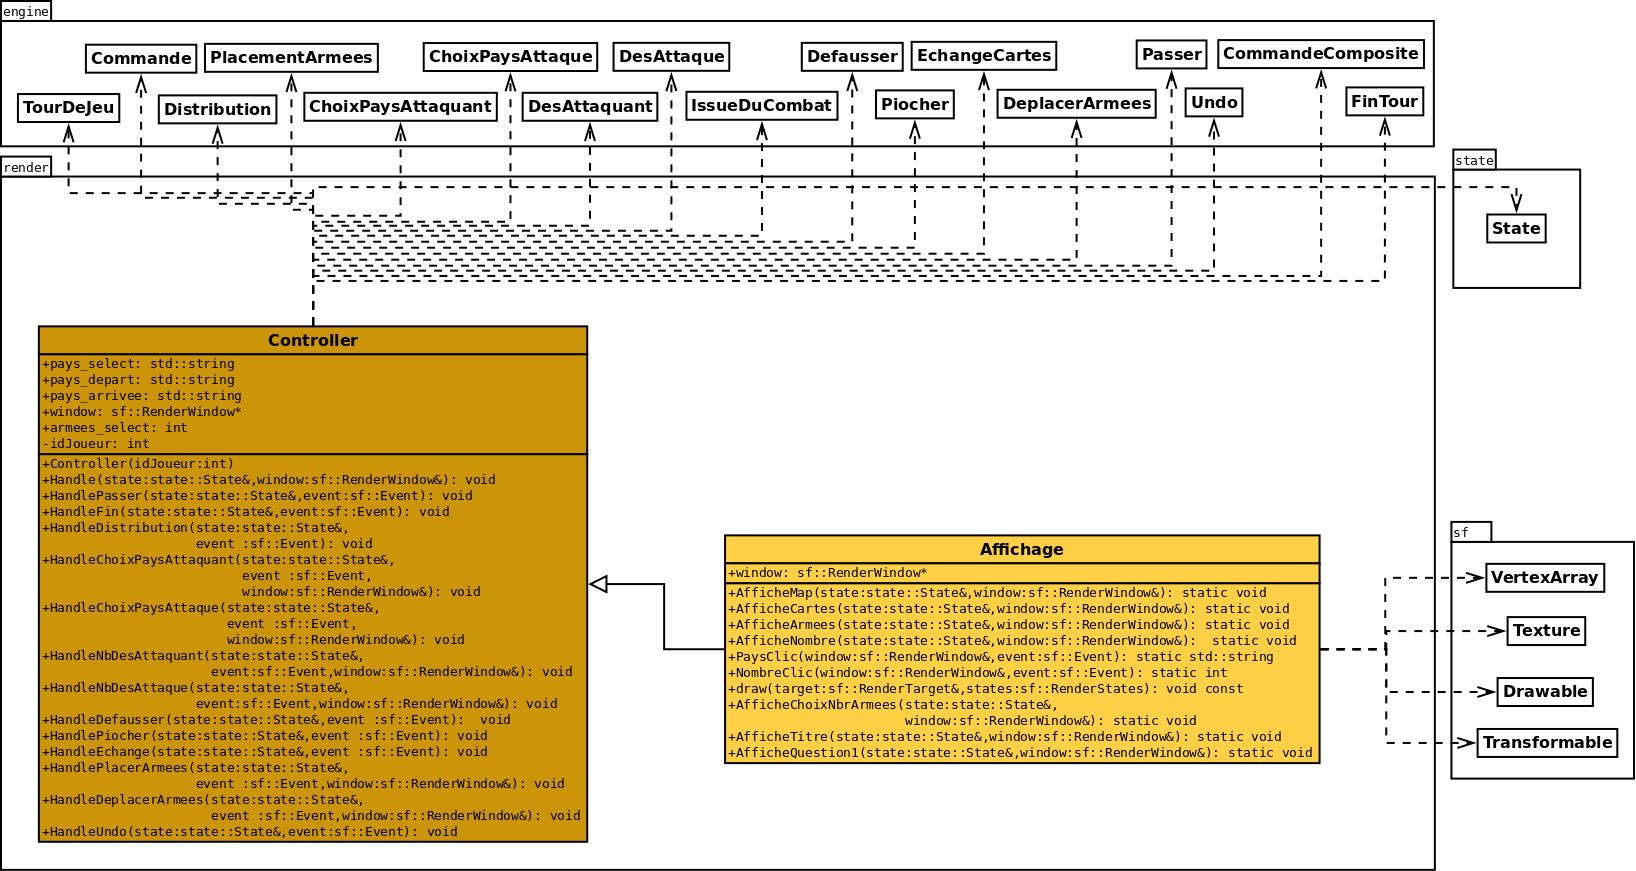
\includegraphics[width=21cm]{Images/render.png}
        \caption{Diagramme des rendus}
        \label{fig:render}
    \end{figure}
\end{landscape}